~\label{section:case-studies:vsmt}
%
\begin{figure}
  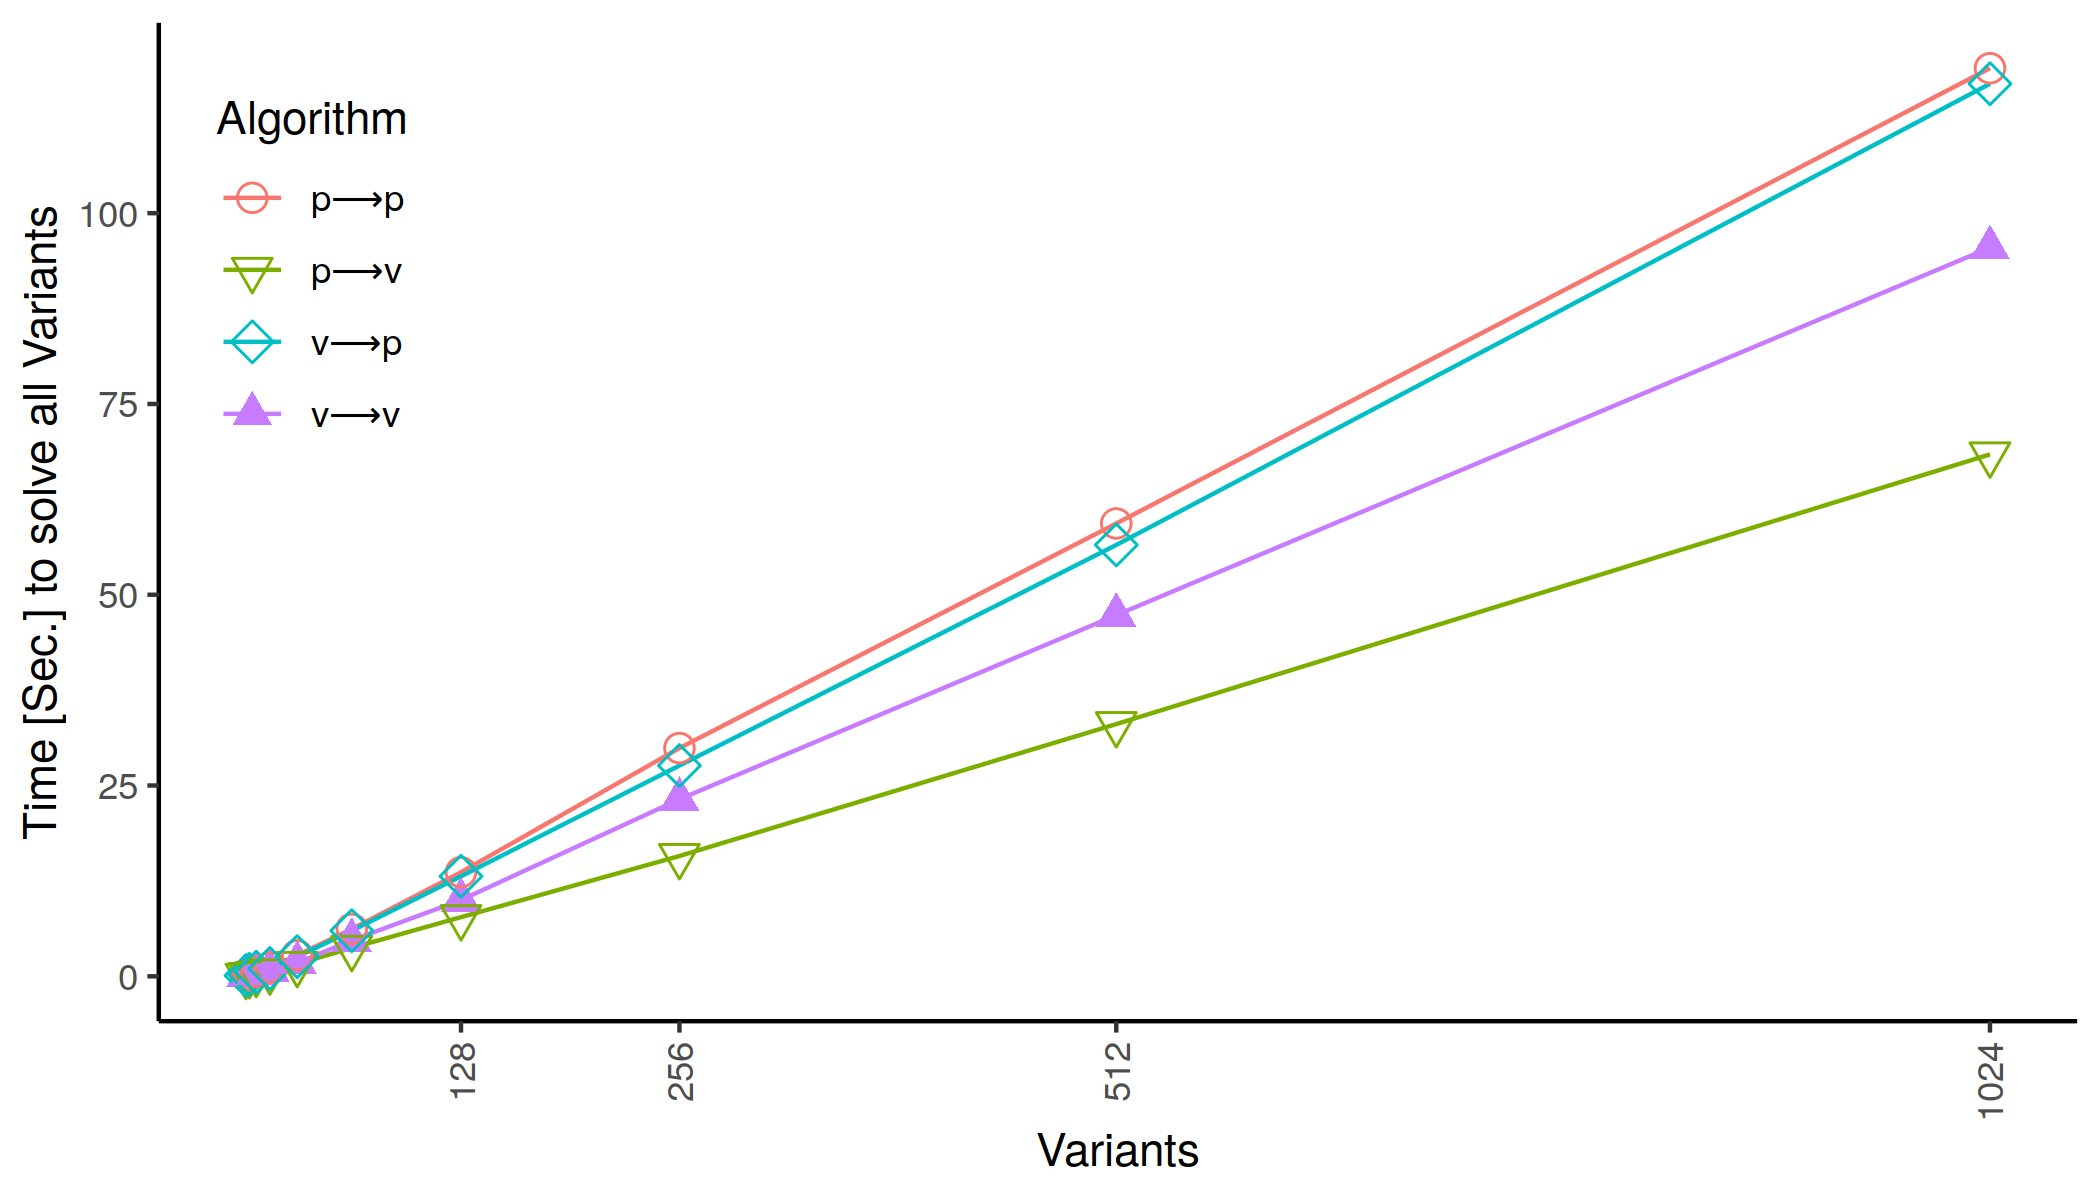
\includegraphics[width=0.95\textwidth]{Plots/RQ1_Fin_Smt}
  \caption{(Financial) Performance as variants increase for the variational
    \ac{smt} solver.}%
  \label{res:rq1:vsmt}
\end{figure}
%
We have shown that the variational \ac{sat} solver exhibits speedup for two
real-world datasets and that the sharing ration of a \ac{vpl} formula is a
significant factor in that speedup. However, we have yet to show that the same
is true for the prototype variational \ac{smt} solver, \vsmt{}.

To test \vsmt{} we use an \ac{smt} version of the \fin{} dataset from \nieke{}'s
study. Unfortunately, only the \fin{} dataset has an \ac{smt} version and so our
evaluation of the prototype \ac{smt} solver is limited. Furthermore, in the
course of encoding the dataset to a \ac{vpl} formula we discovered type errors
in 1,514 formulas out of a total of 4,621 formulas. To utilize the dataset we
detected and corrected the type errors during parsing. The type errors were
essentially identical and revolved around the encoding of a \rn{one-of}
constraint; where only one constraint out of a sequence of constraints can be
true. For example, an incorrect version would be: $(f_{i} \equiv{} 1) \equiv{}
(f_{0} + f_{1} \ldots{} + f_{n})$ for some $i$ and $n$. Thus, the error is that
$f_{i} \equiv 1$ yields a Boolean constraint (\ie{} $\equiv$ has type $\equiv{}
: \eAR{} \rightarrow \eAR{} \rightarrow{} \eIL{}$) but it is the left child of
another $\equiv$ which expects an arithmetic expression as its left child not a
\eIL{} expression. The correction is to repeat $f_{i}$ and handle the boolean
constraint correctly. For example the corrected version of the above formula is
$(f_{i} \equiv{} 1) \wedge{} (f_{i} \equiv{} (f_{0} + f_{1} \ldots{} + f_{n}))$,
where we separate out the left child from the summation but preserve the
semantics of the \rn{one-of} constraint.
